\chapter{Experiments and Results}
\label{ExperimentsAndResults}

\section{Overview}

A conventional pipeline of any deep learning system consists of three main phases: training, prediction, and evaluation. For ease of use and providing more flexibility, a configurable pipeline for this project was implemented. This pipeline was developed in python programming language and is based on the TensorFlow machine learning library. Each experiment in this project, was described in a configuration file. The configuration file specifies the data set, network model, and training parameters used for an experiment. 

New network models and data set drivers can easily be added to the project in form of separate python source code files. By specifying the name of this new models or data sets in a configuration file, the experiment is ready for start; no further changes to the pipeline is required. 

A Linux shell script was used for submitting the experiments to the Advanced Research Computing (ARC3) HPC service provided in University of Leeds. The submitted jobs were executed on Nvidia Tesla P100 GPUs. The time spent for running the experiments varied between 90 minutes to 10 hours per experiment. 

For consistency between results, each model was trained for 100 epochs on the training data set in batches with size of 32 or 16 samples. Most experiments were repeated at least two times to double check the results and the evaluation was performed on a separate test data set. The trained model, predicted normal maps, and evaluation results were stored for each experiment. 

For data augmentation, a per-batch random scaling by factor of 1 or 1.5, random cropping, and random horizontal flipping was performed on the data set samples and the results were resized to the input size of the network. Also, random hue and saturation modifications were applied on images of each batch.   

For consistency with previous research, the loss function used in these experiments is the average of dot products between estimated and desired normal maps over pixels with valid depth data. 

To ensure the quality of software, the source code was developed in interactive Project Jupyter notebooks. Each snippet of code was manually tested and the validity of input and output variable were investigated. The verified changes were committed to a Git repository accessible on GitHub website. On HPC servers, each new model was executed in an interactive session and after confirming the model, the experiments based on that model were sent to scheduler for batch execution. 

The evaluation metrics and the results of experiments are discussed in following sections.

\pagebreak

\section{Metrics}

The metrics used for evaluation of the outputs in this project, are the same metrics used in related work discussed in section \ref{sec:relatedwork}. As mentioned before, by doing so, it is very easy to compare the result of this project with state of the art models. 

Seven metrics are defined for the evaluation of the output of a network. All of them, are based on an error value. To compute this error value, the dot product between normalised predicted normal maps and the desired normal maps for all the samples of the test data set is calculated. Then, the arc cosine function is applied on these values, and the result is converted to degree. In other words, the angle between the corresponding normal vectors in estimated normal maps and desired normal maps is computed in degree. Then the following metrics are calculated based on these angles over the valid pixels in the data set. 

\begin{itemize}
    \item \emph{Mean}: the average of angles between normal vectors
    \item \emph{Median}: the median of angles between normal vectors
    \item \emph{RMSE}: $\sqrt{\frac{1}{n}\sum_{i=1}^{n}E_{i}^{2}}$ , for E= angle between normal vectors and n= number of valid pixels in data set
    \item \emph{\ang{11.25} Error}: the percentage of valid vectors with angles less than \ang{11.25}
    \item \emph{\ang{22.5} Error}: the percentage of valid vectors with angles less than \ang{22.5}
    \item \emph{\ang{30} Error}: the percentage of valid vectors with angles less than \ang{30}
    \item \emph{\ang{45} Error}: the percentage of valid vectors with angles less than \ang{45}
\end{itemize}

\section{Quantitative results}

The result of experiments are illustrated in table \ref{tab:results}. Based on the results obtained from several times training the baseline model with same configuration, a difference more than one percent in \ang{11.25} error is statistically significant.  

\begin{table}[h]
\centering
\begin{tabular}{cccccccc}
Experiment & Mean & Median & RMSE & \ang{11.25} & \ang{22.5} & \ang{30} & \ang{45} \\
\hline
\hline
Baseline & 43.5 & 39.7 & 51.0 & 11.2 & 27.3 & 37.6 & 56.5 \\
12 Conv. Filters & 43.6 & 39.4 & 51.3 & 11.6 & 27.7 & 38.1 & 56.6 \\
15x15 Conv. Kernel & 43.1 & 39.5 & 50.5 & 10.7 & 27.0 & 37.7 & 56.8 \\
Avg. Pooling & 43.8 & 40.2 & 51.1 & 9.9 & 26.0 & 36.7 & 56.0 \\
Larger FC1 & 43.8 & 40.0 & 51.2 & 10.1 & 26.2 & 36.9 & 56.1 \\
Larger FC2 & 43.0 & 39.1 & 50.5 & 11.3 & 27.7 & 38.2 & 57.2 \\
No FC1 & 47.5 & 43.5 & 55.2 & 9.0 & 24.4 & 34.1 & 51.7 \\
Up Sampling & 40.4 & 37.1 & 47.3 & 11.9 & 29.0 & 40.3 & 60.4 \\
\hline
VGG16 & 40.7 & 36.4 & 48.5 & 13.8 & 31.1 & 41.8 & 60.6 \\
VGG Low & 44.1 & 40.1 & 52.0 & 10.9 & 27.0 & 37.3 & 55.9 \\
VGG Mid & 42.2 & 37.2 & 50.5 & 13.6 & 30.8 & 41.2 & 59.0 \\
VGG High & 43.0 & 38.1 & 51.0 & 12.0 & 29.2 & 39.8 & 58.0 \\
VGG Concat. & 48.5 & 44.4 & 55.0 & 4.7 & 17.5 & 28.7 & 50.9 \\
\hline
ResNet50 & 45.0 & 41.6 & 50.5 & 4.7 & 17.5 & 29.6 & 55.3 \\
\hline
Baseline NYU & 42.2 & 38.2 & 50.0 & 12.3 & 28.5 & 39.2 & 58.7 \\
Baseline SUN & 45.2 & 42.2 & 52.7 & 10.5 & 24.9 & 34.7 & 53.5 \\
VGG16 NYU & 41.0 & 37.7 & 47.9 & 10.6 & 27.3 & 38.8 & 60.4 \\
VGG16 SUN & 42.2 & 38.4 & 50.0 & 13.0 & 29.0 & 39.4 & 58.2 \\
\hline
\citeauthor*{wang} \cite{wang} & 25.0 & 13.8 & 35.9 & 44.2 & 63.2 & 70.3 \\
\citeauthor*{eigen}\cite{eigen} & 23.7 & 15.5 & - & 39.2 & 62.0 & 71.1 \\
\citeauthor*{dharmasiri}\cite{dharmasiri} & 20.6 & 13.0 & - & 44.9 & 67.7 & 76.3 \\
\citeauthor*{bansal}\cite{bansal} & 19.8 & 12.0 & 28.2 & 47.9 & 70.0 & 77.8 \\
\end{tabular}
\caption{Quantitative results of evaluation}
\label{tab:results}
\end{table}

\section{Qualitative results}

Figures \ref{fig:baseline1} and \ref{fig:baseline2} illustrate some of the better results obtained by training the baseline model on the main data set. The results of training the VGG16 model on SUN RGB-D based data set are depicted in figures \ref{fig:sunvgg1} and \ref{fig:sunvgg2}. Generally the models perform their best in scenes with a few big and simple objects like beds or tables. 

For comparison, the qualitative results of relevant work to this project is also included (figure \ref{fig:others}). It is clear that there is a big difference between the results obtained in this project and the state of the art. 

\pagebreak

\begin{figure}
    \centering
    \begin{subfigure}[b]{0.3\textwidth}
        \includegraphics[width=\textwidth]{Baseline/25}
    \end{subfigure}
    \begin{subfigure}[b]{0.3\textwidth}
        \includegraphics[width=\textwidth]{Baseline/30}
    \end{subfigure}
    \begin{subfigure}[b]{0.3\textwidth}
        \includegraphics[width=\textwidth]{Baseline/89}
    \end{subfigure}
    
    \begin{subfigure}[b]{0.3\textwidth}
        \includegraphics[width=\textwidth]{Baseline/99}
    \end{subfigure}
    \begin{subfigure}[b]{0.3\textwidth}
        \includegraphics[width=\textwidth]{Baseline/215}
    \end{subfigure}
    \begin{subfigure}[b]{0.3\textwidth}
        \includegraphics[width=\textwidth]{Baseline/219}
    \end{subfigure}
    \caption{Baseline model trained on main data set: \\ RGB images, ground truth normal maps, and estimated normal maps}
    \label{fig:baseline1}
\end{figure}

\begin{figure}
    \centering
    \begin{subfigure}[b]{0.3\textwidth}
        \includegraphics[width=\textwidth]{SUNVGG16/25}
    \end{subfigure}
    \begin{subfigure}[b]{0.3\textwidth}
        \includegraphics[width=\textwidth]{SUNVGG16/30}
    \end{subfigure}
    \begin{subfigure}[b]{0.3\textwidth}
        \includegraphics[width=\textwidth]{SUNVGG16/89}
    \end{subfigure}
    
    \begin{subfigure}[b]{0.3\textwidth}
        \includegraphics[width=\textwidth]{SUNVGG16/99}
    \end{subfigure}
    \begin{subfigure}[b]{0.3\textwidth}
        \includegraphics[width=\textwidth]{SUNVGG16/215}
    \end{subfigure}
    \begin{subfigure}[b]{0.3\textwidth}
        \includegraphics[width=\textwidth]{SUNVGG16/219}
    \end{subfigure}
    \caption{VGG16 model trained on SUN data set: \\ RGB images, ground truth normal maps, and estimated normal maps}
    \label{fig:sunvgg1}
\end{figure}

\begin{figure}
    \centering
    \begin{subfigure}[b]{0.3\textwidth}
        \includegraphics[width=\textwidth]{Baseline/263}
    \end{subfigure}
    \begin{subfigure}[b]{0.3\textwidth}
        \includegraphics[width=\textwidth]{Baseline/271}
    \end{subfigure}
    \begin{subfigure}[b]{0.3\textwidth}
        \includegraphics[width=\textwidth]{Baseline/335}
    \end{subfigure}
    
    \begin{subfigure}[b]{0.3\textwidth}
        \includegraphics[width=\textwidth]{Baseline/401}
    \end{subfigure}
    \begin{subfigure}[b]{0.3\textwidth}
        \includegraphics[width=\textwidth]{Baseline/460}
    \end{subfigure}
    \begin{subfigure}[b]{0.3\textwidth}
        \includegraphics[width=\textwidth]{Baseline/492}
    \end{subfigure}
    \caption{Baseline model trained on main data set: \\ RGB images, ground truth normal maps, and estimated normal maps}
    \label{fig:baseline2}
\end{figure}

\begin{figure}
    \centering
    \begin{subfigure}[b]{0.3\textwidth}
        \includegraphics[width=\textwidth]{SUNVGG16/263}
    \end{subfigure}
    \begin{subfigure}[b]{0.3\textwidth}
        \includegraphics[width=\textwidth]{SUNVGG16/271}
    \end{subfigure}
    \begin{subfigure}[b]{0.3\textwidth}
        \includegraphics[width=\textwidth]{SUNVGG16/335}
    \end{subfigure}
    
    \begin{subfigure}[b]{0.3\textwidth}
        \includegraphics[width=\textwidth]{SUNVGG16/401}
    \end{subfigure}
    \begin{subfigure}[b]{0.3\textwidth}
        \includegraphics[width=\textwidth]{SUNVGG16/460}
    \end{subfigure}
    \begin{subfigure}[b]{0.3\textwidth}
        \includegraphics[width=\textwidth]{SUNVGG16/492}
    \end{subfigure}
    \caption{VGG16 model trained on SUN data set: \\ RGB images, ground truth normal maps, and estimated normal maps}
    \label{fig:sunvgg2}
\end{figure}


\begin{figure}
    \centering
    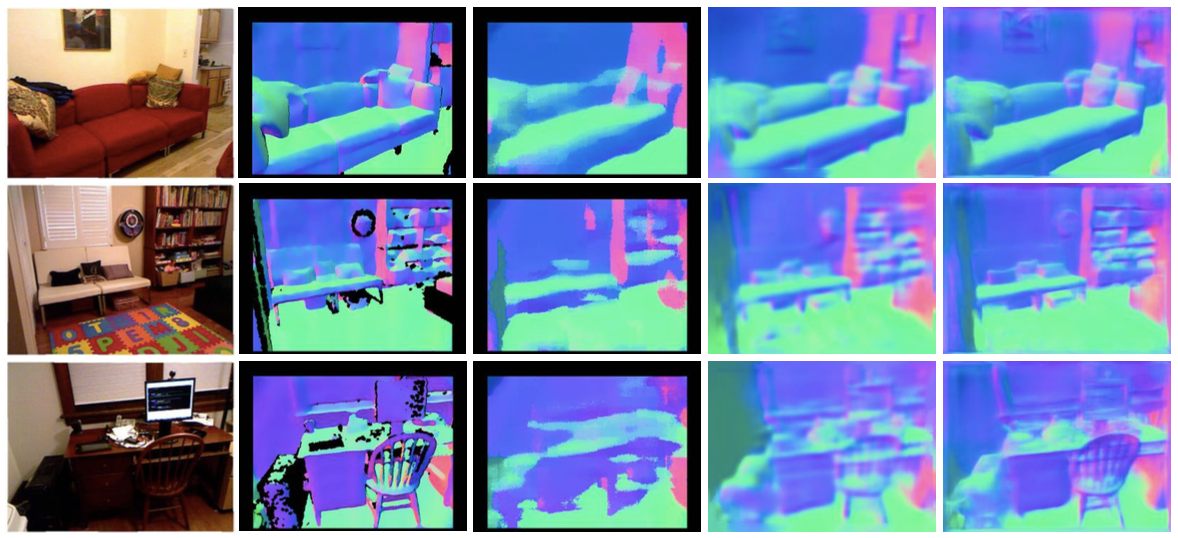
\includegraphics[width=\textwidth]{Others}
    \caption{From left to right: RGB images, ground truth normal maps, \\ qualitative results of \citeauthor*{wang}, \citeauthor*{eigen}, and \citeauthor*{bansal} }
    \label{fig:others}
\end{figure}

